\clearpage
\section{Experimental validation on a linear axis}
\label{sec:ExperimentalValidation}

The experimental validation reported in the previous \autoref{sec:shaker_test01} and \autoref{sec:shaker_test02} was carried out in a well-controlled envinronment with a shaker that was able to generate vibration according to specific references. To further test the framework, a real-word application is considered in this section. The setup consists of a machine equipped with a linear axis, that is used to move a platform. On the emoving platform the same accelerometer described in \autoref{tab:adxl335_specifications} has been atached using a custom 3D-printed fixture.

The test consists of defining a set of movements to be actuated by the platform, the accelerometer is used to capture the characteristics of each movement. As it has done previously, some movement profiles are used for training and some other for testing. The position reference is shown in \autoref{fig:etel_profile}, and the parameters of the profiles are resumed in \autoref{tab:etel_profiles}.

\begin{figure}
    \centering
    \todo%\includegraphics{Images/etel/etel_profile.pdf}
    \caption{Position reference for the linear axis test.}
    \label{fig:etel_profile}
\end{figure}

\begin{table}
    \centering
    \caption{Harmonic coefficients for the shaker test.}
    \label{tab:etel_profiles}
    \begin{tabular}{cccc} 
    \toprule
    \textbf{Profile N.} & \textbf{Speed} {[}$\text{m}\text{s}^{-1}$] & \textbf{Acceleration} {[}$\text{m}\text{s}^{-2}$] & \textbf{Jerk} {[}$\text{s}$] \\ 
    \hline
    1 & 0.8 & 6 & 0.02 \\
    2 & 0.4 & 3 & 0.02 \\
    3 & 0.4 & 6 & 0.02 \\
    4 & 0.6 & 8 & 0.02 \\
    \bottomrule
\end{tabular}
\end{table}

\subsection{Training}
To perform the training, a loop has been implemented on the \gls{pc} that managed the axis movements. The script cyclically actuates the axis to follow the reference profile, and ask the microcontroller to start the acquisition of the accelerometer data. The received features are then stored in a file, and the process is repeated for each profile. The sampling frequency of the microcontroller is 5kHz, for a total of 6000 samples per profile. 

Although not useful for the training, the microcontroller has been set to not only transmit the features to the \gls{pc}, but also the timeseries, for visualization purposes. The timeseries of the training set are shown in \autoref{fig:axis_timeseries}, and the features are shown in \autoref{fig:axis_features}.

In the timeseries set if is possible to see some outliers, for example there is a record in wich the profile 1 started being actuated by the axis with a delaty \gls{wrt} the others. Profile 4, instead, has some outliers due to the axix sometimes overshooting the reference position.

The training set is containing 100 snapshots for each profile, for a total of 400 snapshots. The K-means model is then trained for $n=5$ clusters, accordingly with the silhouette criterion.

\begin{figure}
    \centering
    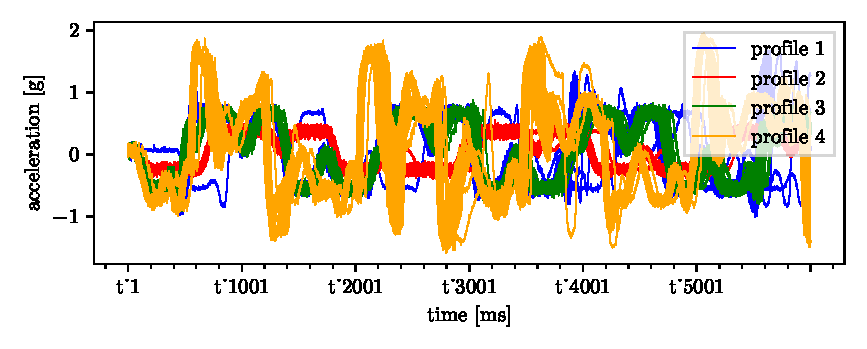
\includegraphics{images/LinearMotor/Timeseries.pdf}
    \caption{Timeseries of the training set}
    \label{fig:axis_timeseries}
\end{figure}


\begin{figure}
    \centering
    \includegraphics[width=\textwidth]{images/LinearMotor/Features.pdf}
    \caption{features of the training set}
    \label{fig:axis_features}
\end{figure}

As done previously, the training is performed with the user confirming the correct number of clusters. And updating the model into the microcontroller.

\subsection{Testing}
The microcontroller is them set in \emph{evaluate} mode and the \gls{nd} is performed on a loop that repeated the movement of profile 2. The result of this first model (Model 1) is shown in \autoref{fig:axis_testing}. We can see that the model immediately falsely detect a novelty, despite the profile 2 was part of the training set. The figure also shows a cleaned view of the evolution of the novelty score, obtained by applying a moving average filter on the last 5 values ov the novelty metric.

Let's investigate why this model gives almost all false positive results. Analyzing the features of the training set (\autoref{fig:axis_features}), we can see that the firt features, up to $\approx 12$, are grouped by profile, but most of the remaining features are not, this arises the suspect that theese features may not be significative of the movement, but maybe just representing noise. This is likely also because the necessary standardization procedure ensure that each feature will have unitary standard deviation, regardless of the magnitude of the feature itself \gls{wrt} the others. This may cause \quoted{noise} features to be amplifigated in the model. Moreover, it's clear that being most of the features not significative, the model is not able to distinguish between the profiles.

\subsection{Feature scaling}
To address the problem of the non-significative features, a feature scaling method is proposed. The idea is to scale the features in such a way that the most significative features will have a higher weight in the model. To do that, a naive approach could be visually select the important features (by eye it's evident that are the first few) and apply a small scaling factor to the others. 

This approach goes against the principle of the framework being fully automatic to train. To address this problem, an unsupervised and automatic method is proposed. The idea is to scale the features in such a way that the most significative features will have a higher weight in the model. To do that, it's possible to exploit the fact that, at this point, the K-means model is already trained and this step provided lables for the training dataset. It's now possible to apply a \emph{supervised} \gls{ml} algorithm in a way that is transparent to the user, so the whole procedure remain \emph{unsupervised}.

Luckily, the \gls{sklearn} library provides a method 


\begin{figure}
    \centering
    %\includegraphics{images/LinearMotor/Testing.pdf}
    \caption{Novelty detection on profile 2.}
    \label{fig:axis_testing}
\end{figure}